
\chapter{Apache Cordova}

The \href{https://cordova.apache.org}{Apache Cordova} is one of the best known technologies to create modern cross-platform mobile applications. This framework allows to create applications using standard HTML5 technologies stack in order to build mobile apps for Android and iOS mobile devices. The requirements for developer is the knowledge of classical technologies like html, css and JavaScript.

In order to begin work with Cordova environment we have to install \href{http://nodejs.org}{Node.js} application. \begin{warning} This will require administrator privileges on the system.\end{warning} The Node.js environment contains npm - nodejs packet manager that allow to install new packages/application into our system. Using npm we can easily install Cordova by writing in command line:

\begin{shell}
npm install -g cordova
\end{shell}

This -g switch will install cordova for all users, if one wants to install Cordova only for active user we can omit -g parameter.

Now we are ready to create first Cordova app, for that let us create a new directory somewhere in the system and go into this folder.

\begin{shell}
mkdir CordovaApps
cd CordovaApps
\end{shell}

Now we should invoke command:
\begin{shell}
cordova create FirstCordovaApp
\end{shell}

This will create an folder with prepared template of Cordova application. The prepared folder contain few subfolders the most important from the point of view of game developer is www. The rest of subfolders we can treat as internal Cordova folder and let them be.

Just for start we can try to run the project, first we have to add a platform - i.e. the platform we would like to use as deployment machine. In Cordova we have many platforms to choose in this course we will use only Browser for first level debugging, and Android or iOS for second level debugging and final deployment.

\begin{shell}
cd FirstCordovaApp
cordova platform add browser
\end{shell}

And run the created simple starting project

\begin{shell}
cordova run browser
\end{shell}

We should see some information in the terminal and our default browser should open an address \url{http:\\localhost:8000/index.html}. We will see simple page with Cordova logo and a text: device is ready.

Now let us look what is a content of www folder and what lines in the code makes the browser to show this screen \ref{fig.basic_app}.

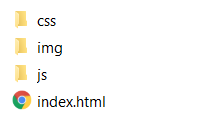
\includegraphics[width=60pt]{chapters/img/basic_structure.png}

We can see specific folders for css, img and js files respectively and one file index.html.

When we open index.html file we will notice the main two parts contained in <head> and <body> tags. At the moment let us ignore <head> part as there is not too many interesting elements and focus on <body>

\begin{html}
<body>
        <div class="app">
            <h1>Apache Cordova</h1>
            <div id="deviceready" class="blink">
                <p class="event listening">Connecting to Device</p>
                <p class="event received">Device is Ready</p>
            </div>
        </div>
        <script type="text/javascript" src="cordova.js"></script>
        <script type="text/javascript" src="js/index.js"></script>
</body>
\end{html}

W can notice few things:
\begin{explain}
\begin{itemize}
\item The JavaScript files are added at the end of the <body> part. This is connected with the order of loading elements in html, and as .js files can operate on html elements it is better to first build these elements before start actions programmed in .js files.

\item We should remember that \begin{warning}cordova.js\end{warning} has to be always the firs script

\item All elements of the web page are contained in one <div class="app"> element

\item There is one <div> element  with id = "deviceready"
\item One <p> element has class listening while the other received

\end{itemize}
\end{explain}

Let us now look into js/index.js file

\jsfile{chapters/code_samples/chapter_cordova_intro/code3.js}

\begin{explain}
How it works: when the page is finally loaded the Cordova environment fire an event 'deviceready', this implies that binded method onDeviceReady is invoked. In the result the method receivedEvent is started with appropriate value of parameter id. In this method the elements with class "listening" becomes invisible while the one with "received" becomes visible.

Explanation line by line:
\begin{description}
\item{line 3:} As we can see in the line 3 the method onDeviceReady is binded to the event 'deviceready'.
\item{line 7:} Run method receivedEvent with parameter id = 'deviceready'
\item{line 11:} Find in the html document the element with id = 'deviceready', store it as parentElement
\item{line 12:} Find all child nodes of parentElement the ones with class "listening", store it as listeningElement
\item{line 13:} Find all child nodes of parentElement the ones with class "received", store it as receivingElement
\item{line 15:} Set style of element listeningElement to display:none, i.e. hide if it is visible on the screen
\item{line 16:} Set style of element receivedElement to display:block, i.e. show if it is not visible on the screen
\item(line 18:) Print a debugging information to JavaScript console.
\item{line 22:} The function initialize of the object app is invoked when javascript is loaded.
\end{description}
\end{explain}

As was mentioned Cordova environment uses a special event 'deviceready'. By default Cordova has more specially defined events, some of them works for all platforms some only for Android (see \url{https://cordova.apache.org/docs/en/latest/cordova/events/events.html}):

\begin{tabularx}{\textwidth}{lX}
'deviceready':& The deviceready event fires when Cordova is fully loaded.\\
'pause': & The pause event fires when the native platform puts the application into the background.\\
'resume':& The resume event fires when the native platform pulls the application out from the background.\\
'backbutton':& The event fires when the user presses the back button.\\
'menubutton':& The event fires when the user presses the menu button. \\
'searchbutton':& The event fires when the user presses the search button on Android. \\
'volumedownbutton':& The event fires when the user presses the volume down button.\\
'volumeupbutton':& The event fires when the user presses the volume up button.\\
\end{tabularx}




